% frontmatter/capitulo-prueba.tex
% Capítulo de PRUEBA de Fase 0 — verifica el flujo completo: recuadro tcolorbox,
% figura TikZ, figura MATLAB exportada y una cita bibliográfica (natbib+apalike).
% No forma parte del libro final; se sustituye por el Cap. 1 real en la Fase 2.

\chapter*{Capítulo de prueba (verificación de andamiaje, Fase 0)}
\addcontentsline{toc}{chapter}{Capítulo de prueba (verificación de andamiaje)}
\progtag{0.0.0}

Este capítulo existe únicamente para verificar, antes de escribir contenido real,
que el flujo \texttt{MATLAB → figura vectorial → \LaTeX{}} y los elementos
tipográficos definidos en \texttt{config/} compilan sin errores.

\begin{cajaDefinicion}
El \textit{customer journey} (recorrido del consumidor) es la secuencia de puntos
de contacto que un consumidor atraviesa desde el reconocimiento de una necesidad
hasta la evaluación posterior a la compra \parencite{solomon2017}.
\end{cajaDefinicion}

\begin{figure}[htbp]
  \centering
  % figuras/tikz/fase0-diagrama-prueba.tex
% Diagrama de prueba (Fase 0): tres etapas simples del recorrido del consumidor.
% Compilable solo (standalone) o incluible con \input en el libro/Beamer.
\begin{tikzpicture}[
    etapa/.style={rectangle, rounded corners, draw=guindaIPN, thick,
                  fill=guindaIPN!8, minimum width=3.1cm, minimum height=1.1cm,
                  align=center, font=\small},
    flecha/.style={-{Stealth[length=2.5mm]}, thick, draw=doradoIPN}
  ]
  \node[etapa] (a) {Reconocimiento\\ de necesidad};
  \node[etapa, right=1.6cm of a] (b) {Búsqueda de\\ información};
  \node[etapa, right=1.6cm of b] (c) {Evaluación\\ posterior};

  \draw[flecha] (a) -- (b);
  \draw[flecha] (b) -- (c);
\end{tikzpicture}

  \caption{Diagrama conceptual de prueba (TikZ). Fuente: elaboración propia.}
  \label{fig:fase0-tikz}
\end{figure}

\begin{figure}[htbp]
  \centering
  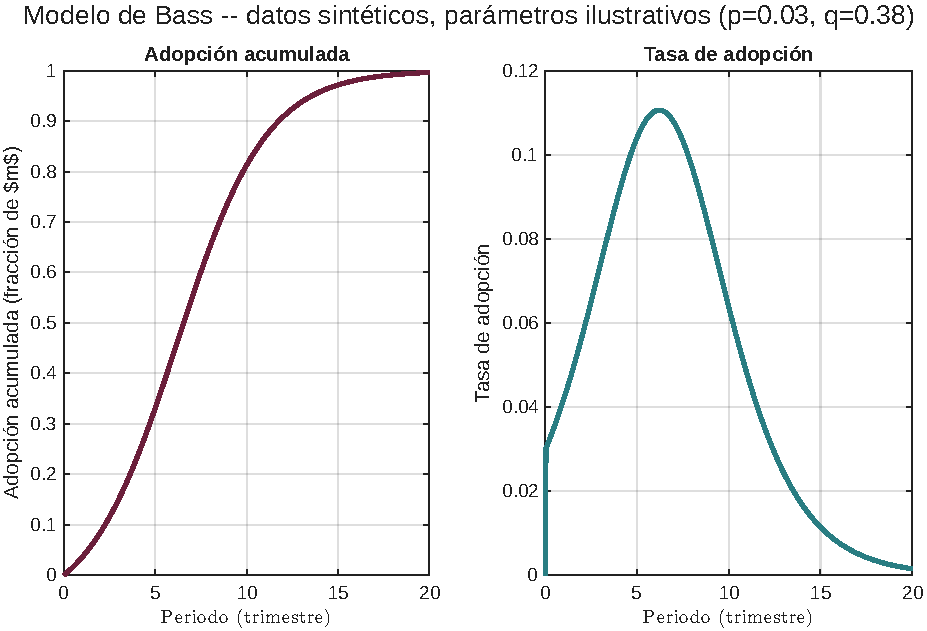
\includegraphics[width=0.9\textwidth]{figuras/matlab/fase0_bass_prueba.pdf}
  \caption{Curva de adopción del modelo de Bass. Fuente: elaboración propia con
  datos sintéticos, \texttt{rng(42)}, parámetros ilustrativos.}
  \label{fig:fase0-matlab}
\end{figure}

\begin{cajaEtica}
Toda cifra de mercado que aparezca en el libro final estará respaldada en
\texttt{docs/verificacion-datos.md}; los datos de esta figura son sintéticos y
están rotulados como tales, conforme al \S5.8 del prompt de proyecto.
\end{cajaEtica}

\pendiente{Sustituir este capítulo por el contenido real del Cap. 1 en la Fase 2.}
